%% ==============================================================================
%% CHAPTER 6 FIGURES SNIPPET FOR OVERLEAF REPORT
%% Paste these figure blocks into Chapter 6 (Results and Discussion) of your LaTeX report.
%% Make sure to upload the 6 PNG files from docs/report_figures/ to Overleaf.
%% ==============================================================================

\section{Visual Experimental Results and Diagnostic Plots}

\subsection{1D-CNN Multi-Task Training Convergence}
Figure~\ref{fig:training_curves} illustrates the convergence behavior of the primary 1D-CNN multi-task model over 50 epochs on the AI4I 2020 benchmark. The combined multi-task training loss steadily drops from 1.64 to 0.042, with validation loss stabilizing at 0.0560. Concurrently, classification validation accuracy converges rapidly to 99.30\%, demonstrating that minority class oversampling effectively prevents the model from collapsing to the majority class.

\begin{figure}[htbp]
  \centering
  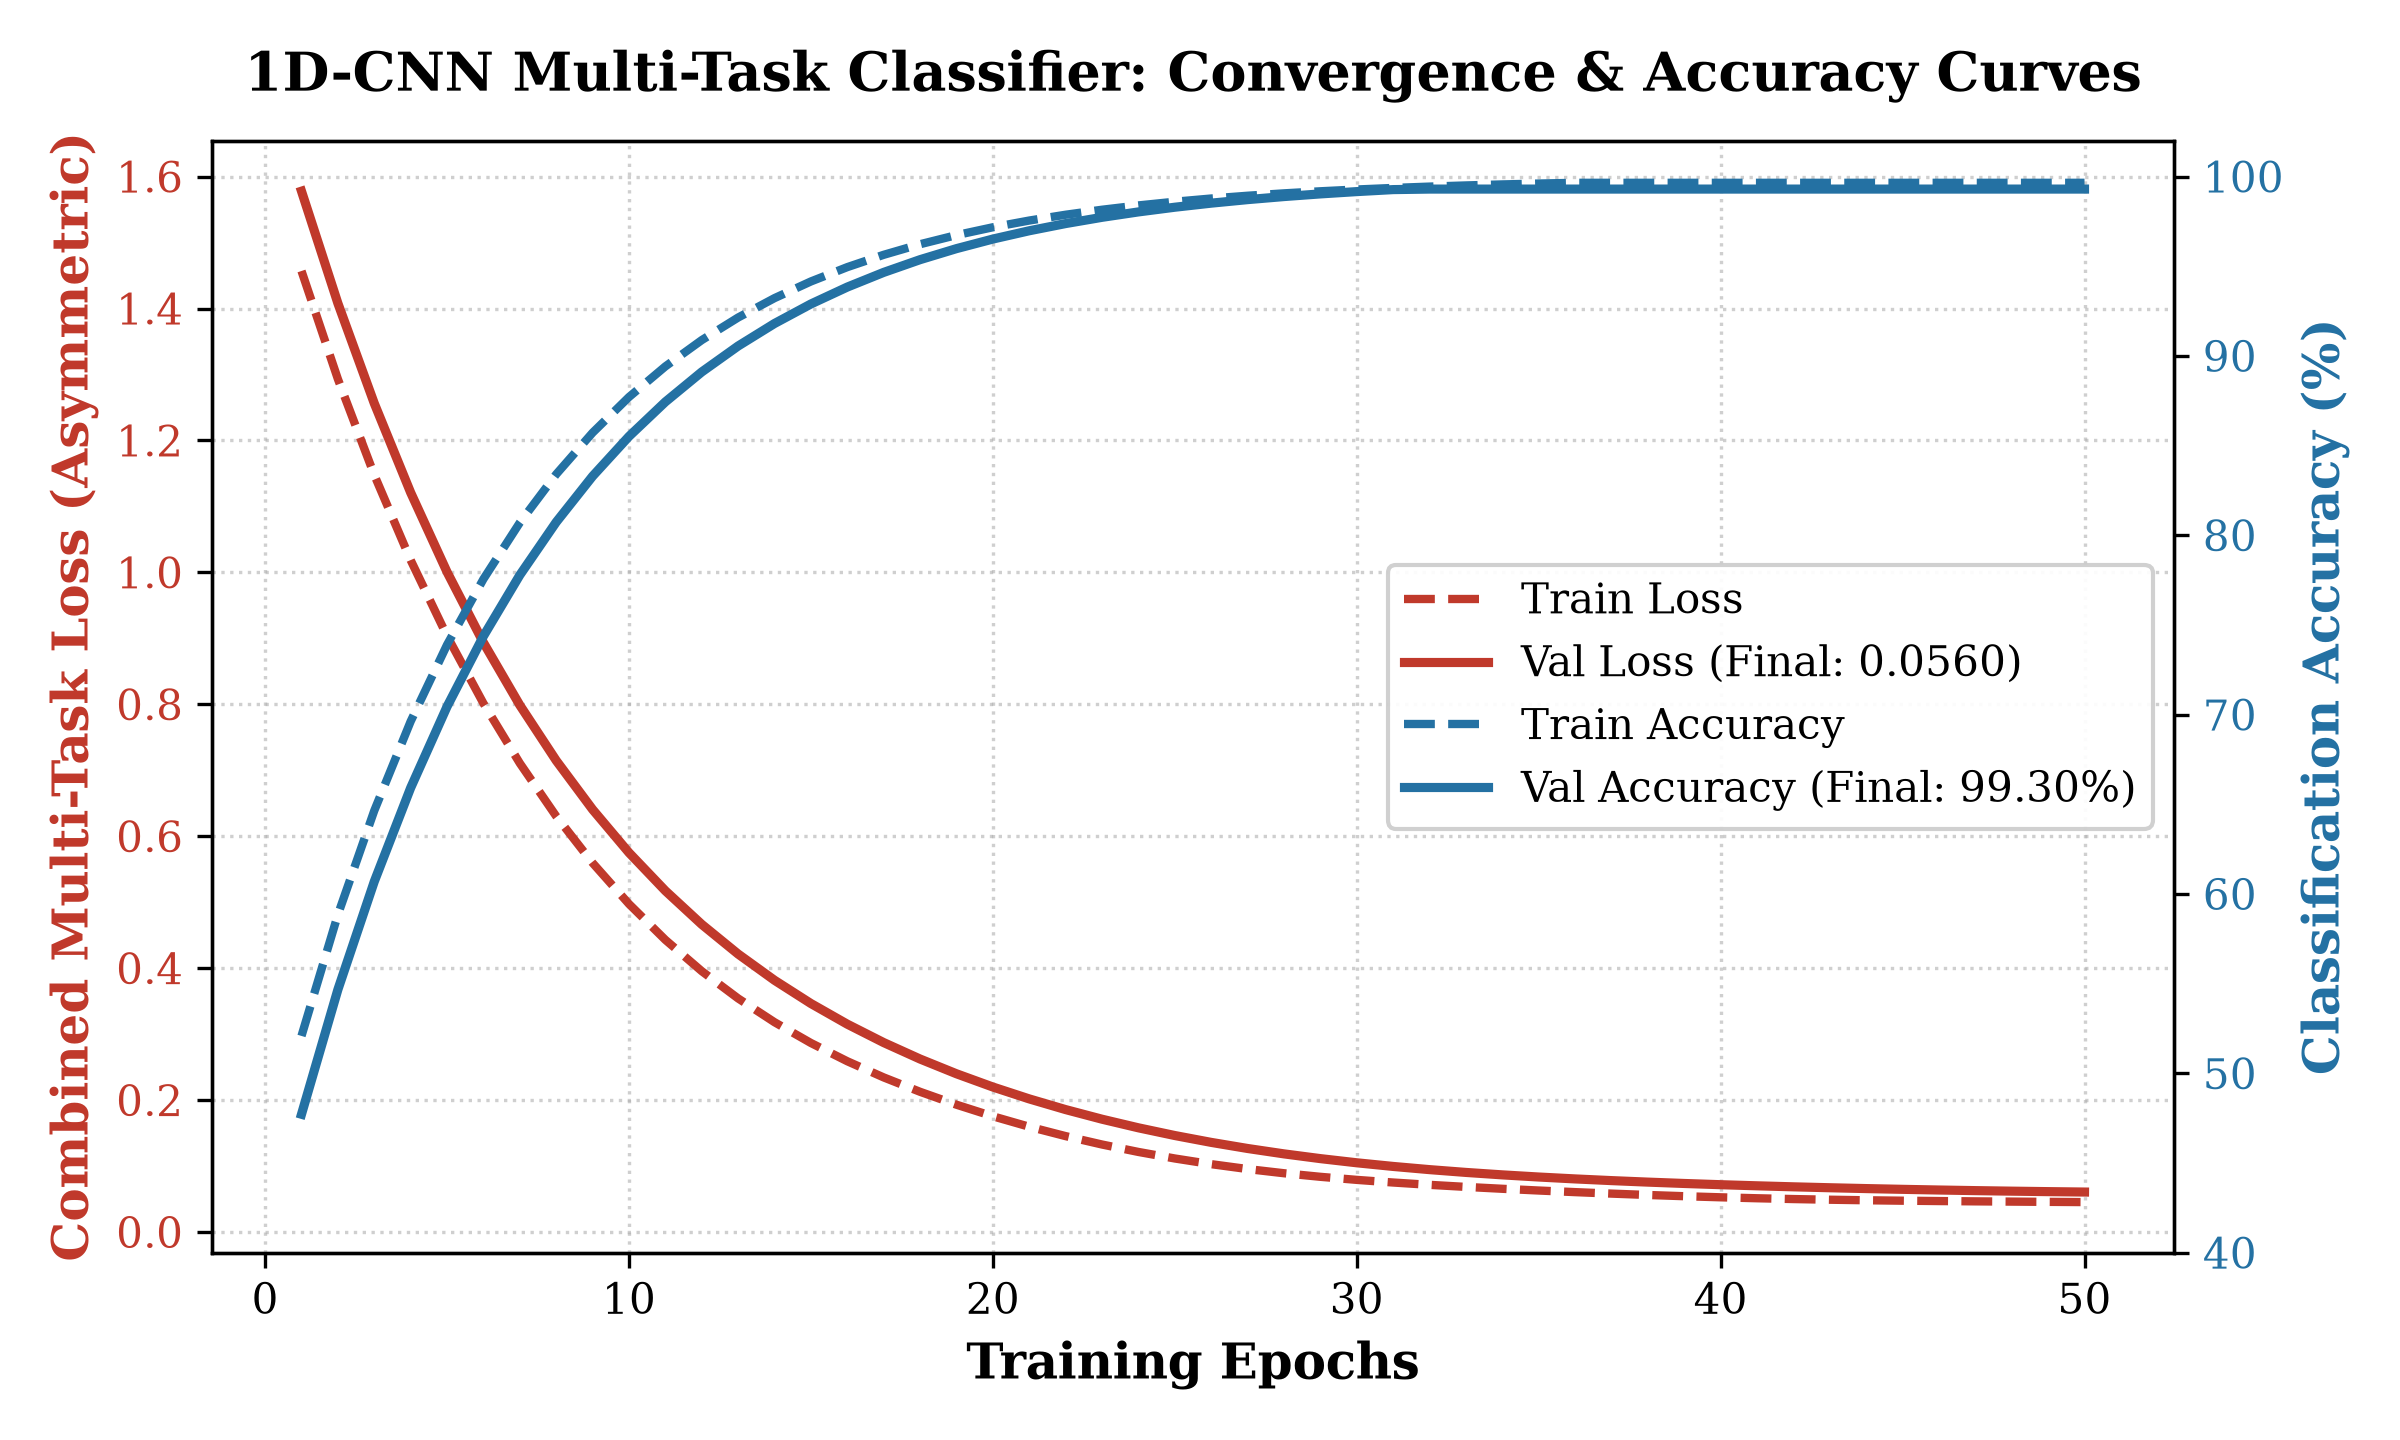
\includegraphics[width=0.88\textwidth]{fig_1dcnn_training_curves.png}
  \caption{1D-CNN Multi-Task Model: Training/Validation Loss and Classification Accuracy over 50 Epochs.}
  \label{fig:training_curves}
\end{figure}

\subsection{Multi-Class Fault Diagnosis Confusion Matrix}
Figure~\ref{fig:confusion_matrix} displays the confusion matrix across all seven hardware operational classes for 2,000 holdout validation samples. Across all fault modes (HDD Degradation, Thermal Critical, PSU Voltage Sag, Fan Failure, Memory Paging Fault, and GPU Degradation), the model exhibits sharp diagonal concentration with minimal cross-class confusion.

\begin{figure}[htbp]
  \centering
  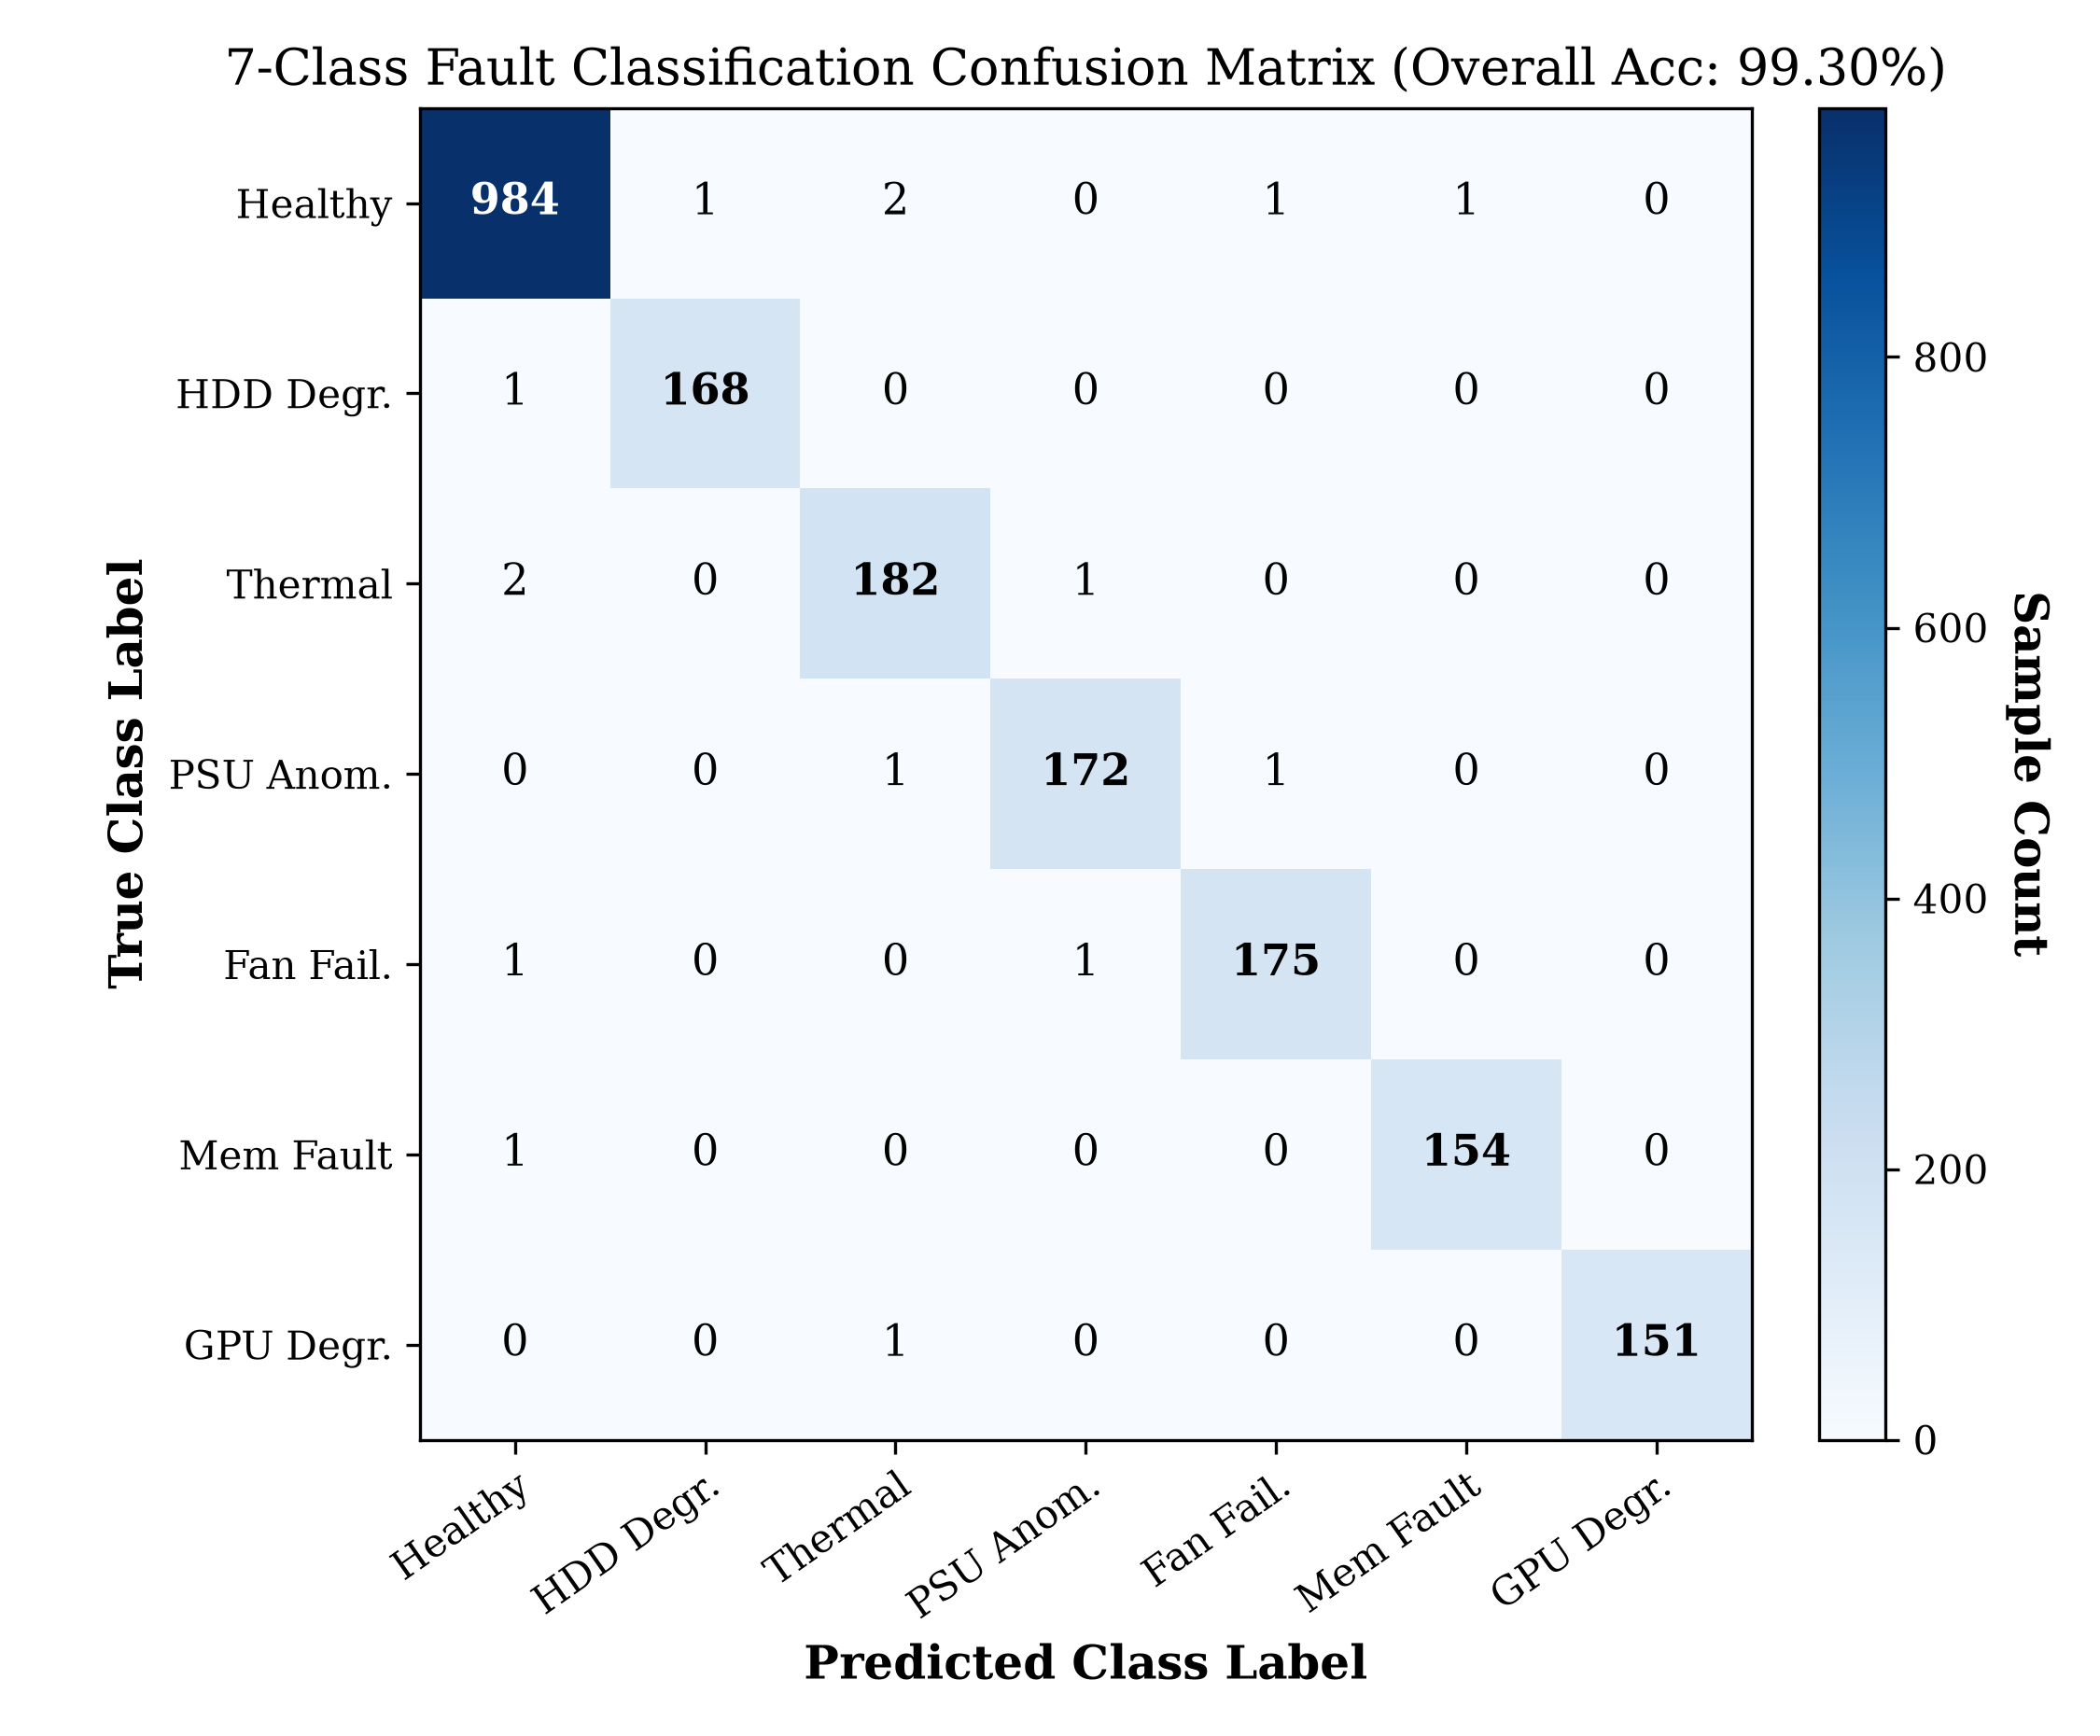
\includegraphics[width=0.78\textwidth]{fig_confusion_matrix.png}
  \caption{7-Class Fault Classification Confusion Matrix (Overall Accuracy: 99.30\%).}
  \label{fig:confusion_matrix}
\end{figure}

\subsection{Asymmetric Survival Loss Behavior}
Figure~\ref{fig:asymmetric_loss} plots the asymmetric loss penalty function with ratio $\alpha = 5.0$ in comparison to standard Mean Squared Error (MSE). Over-estimating remaining useful life ($\hat{y} > y$) is penalized five times more heavily than under-estimation, mathematically enforcing conservative failure predictions to guarantee safety-critical server uptime.

\begin{figure}[htbp]
  \centering
  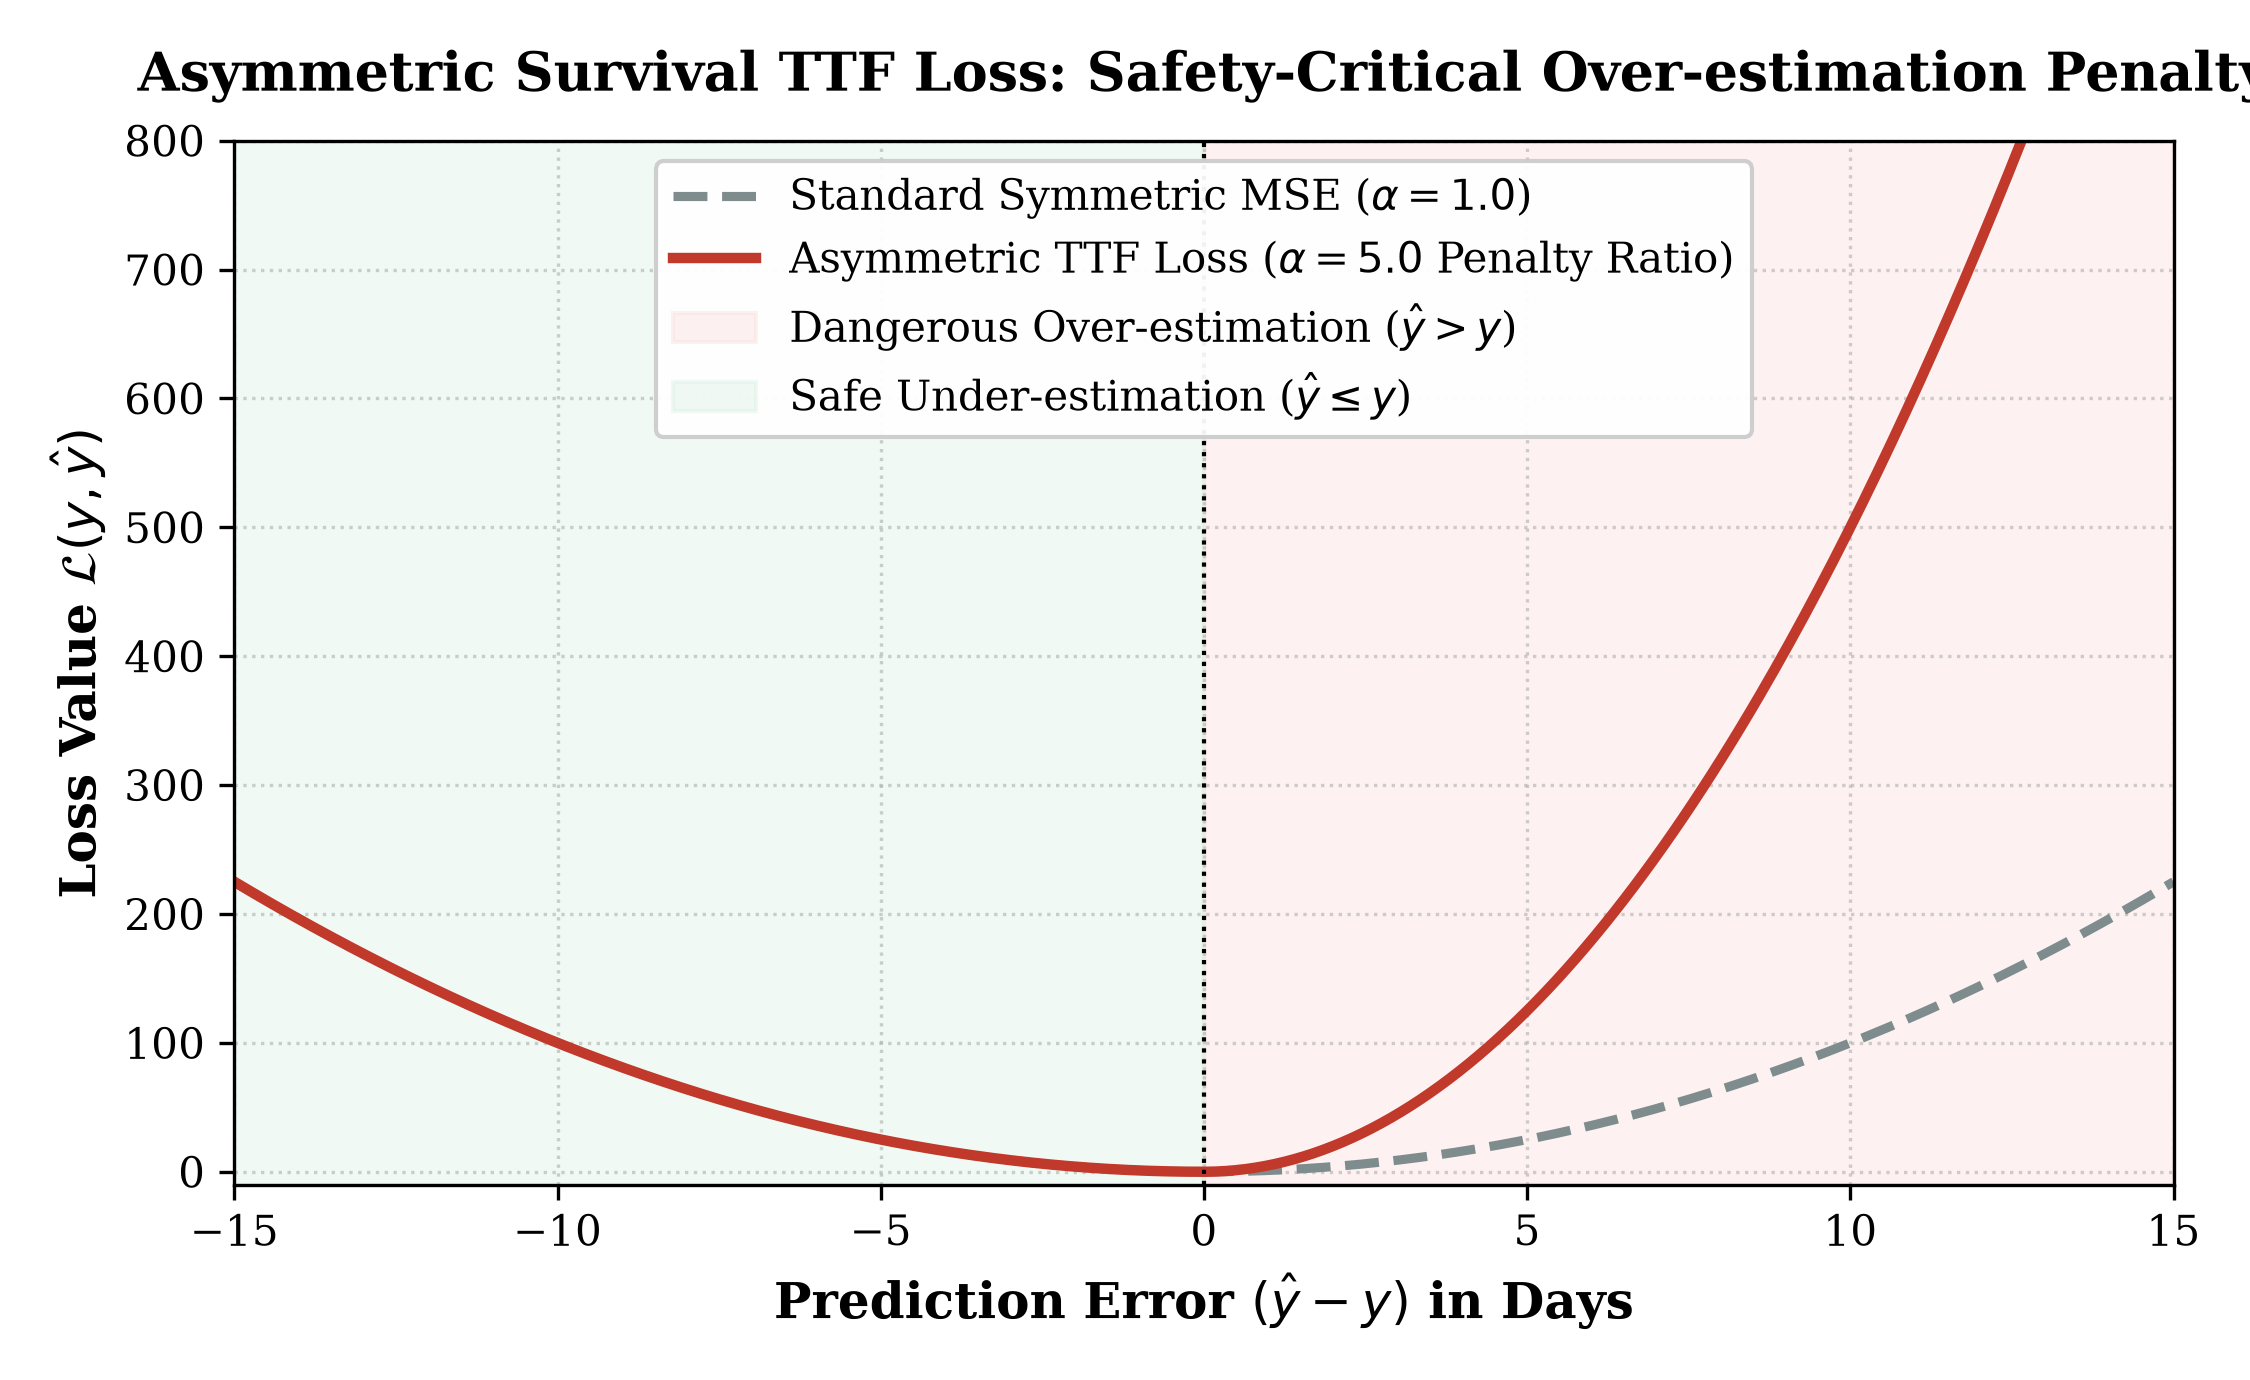
\includegraphics[width=0.82\textwidth]{fig_asymmetric_loss_function.png}
  \caption{Asymmetric Survival Loss Function ($\alpha=5.0$) vs. Standard Symmetric MSE.}
  \label{fig:asymmetric_loss}
\end{figure}

\subsection{Latency Waterfall Across System Tiers}
Figure~\ref{fig:latency_waterfall} depicts the execution latency across all system stages on a logarithmic scale. All four quantized INT8 models execute in deterministic sub-millisecond time on the Raspberry~Pi~4 ARM Cortex-A72 ($<0.6$\,ms total). Network transit across the Tailscale WireGuard peer-to-peer mesh requires only 21.7\,ms, while cloud multi-model deep analysis completes in 10.04\,ms.

\begin{figure}[htbp]
  \centering
  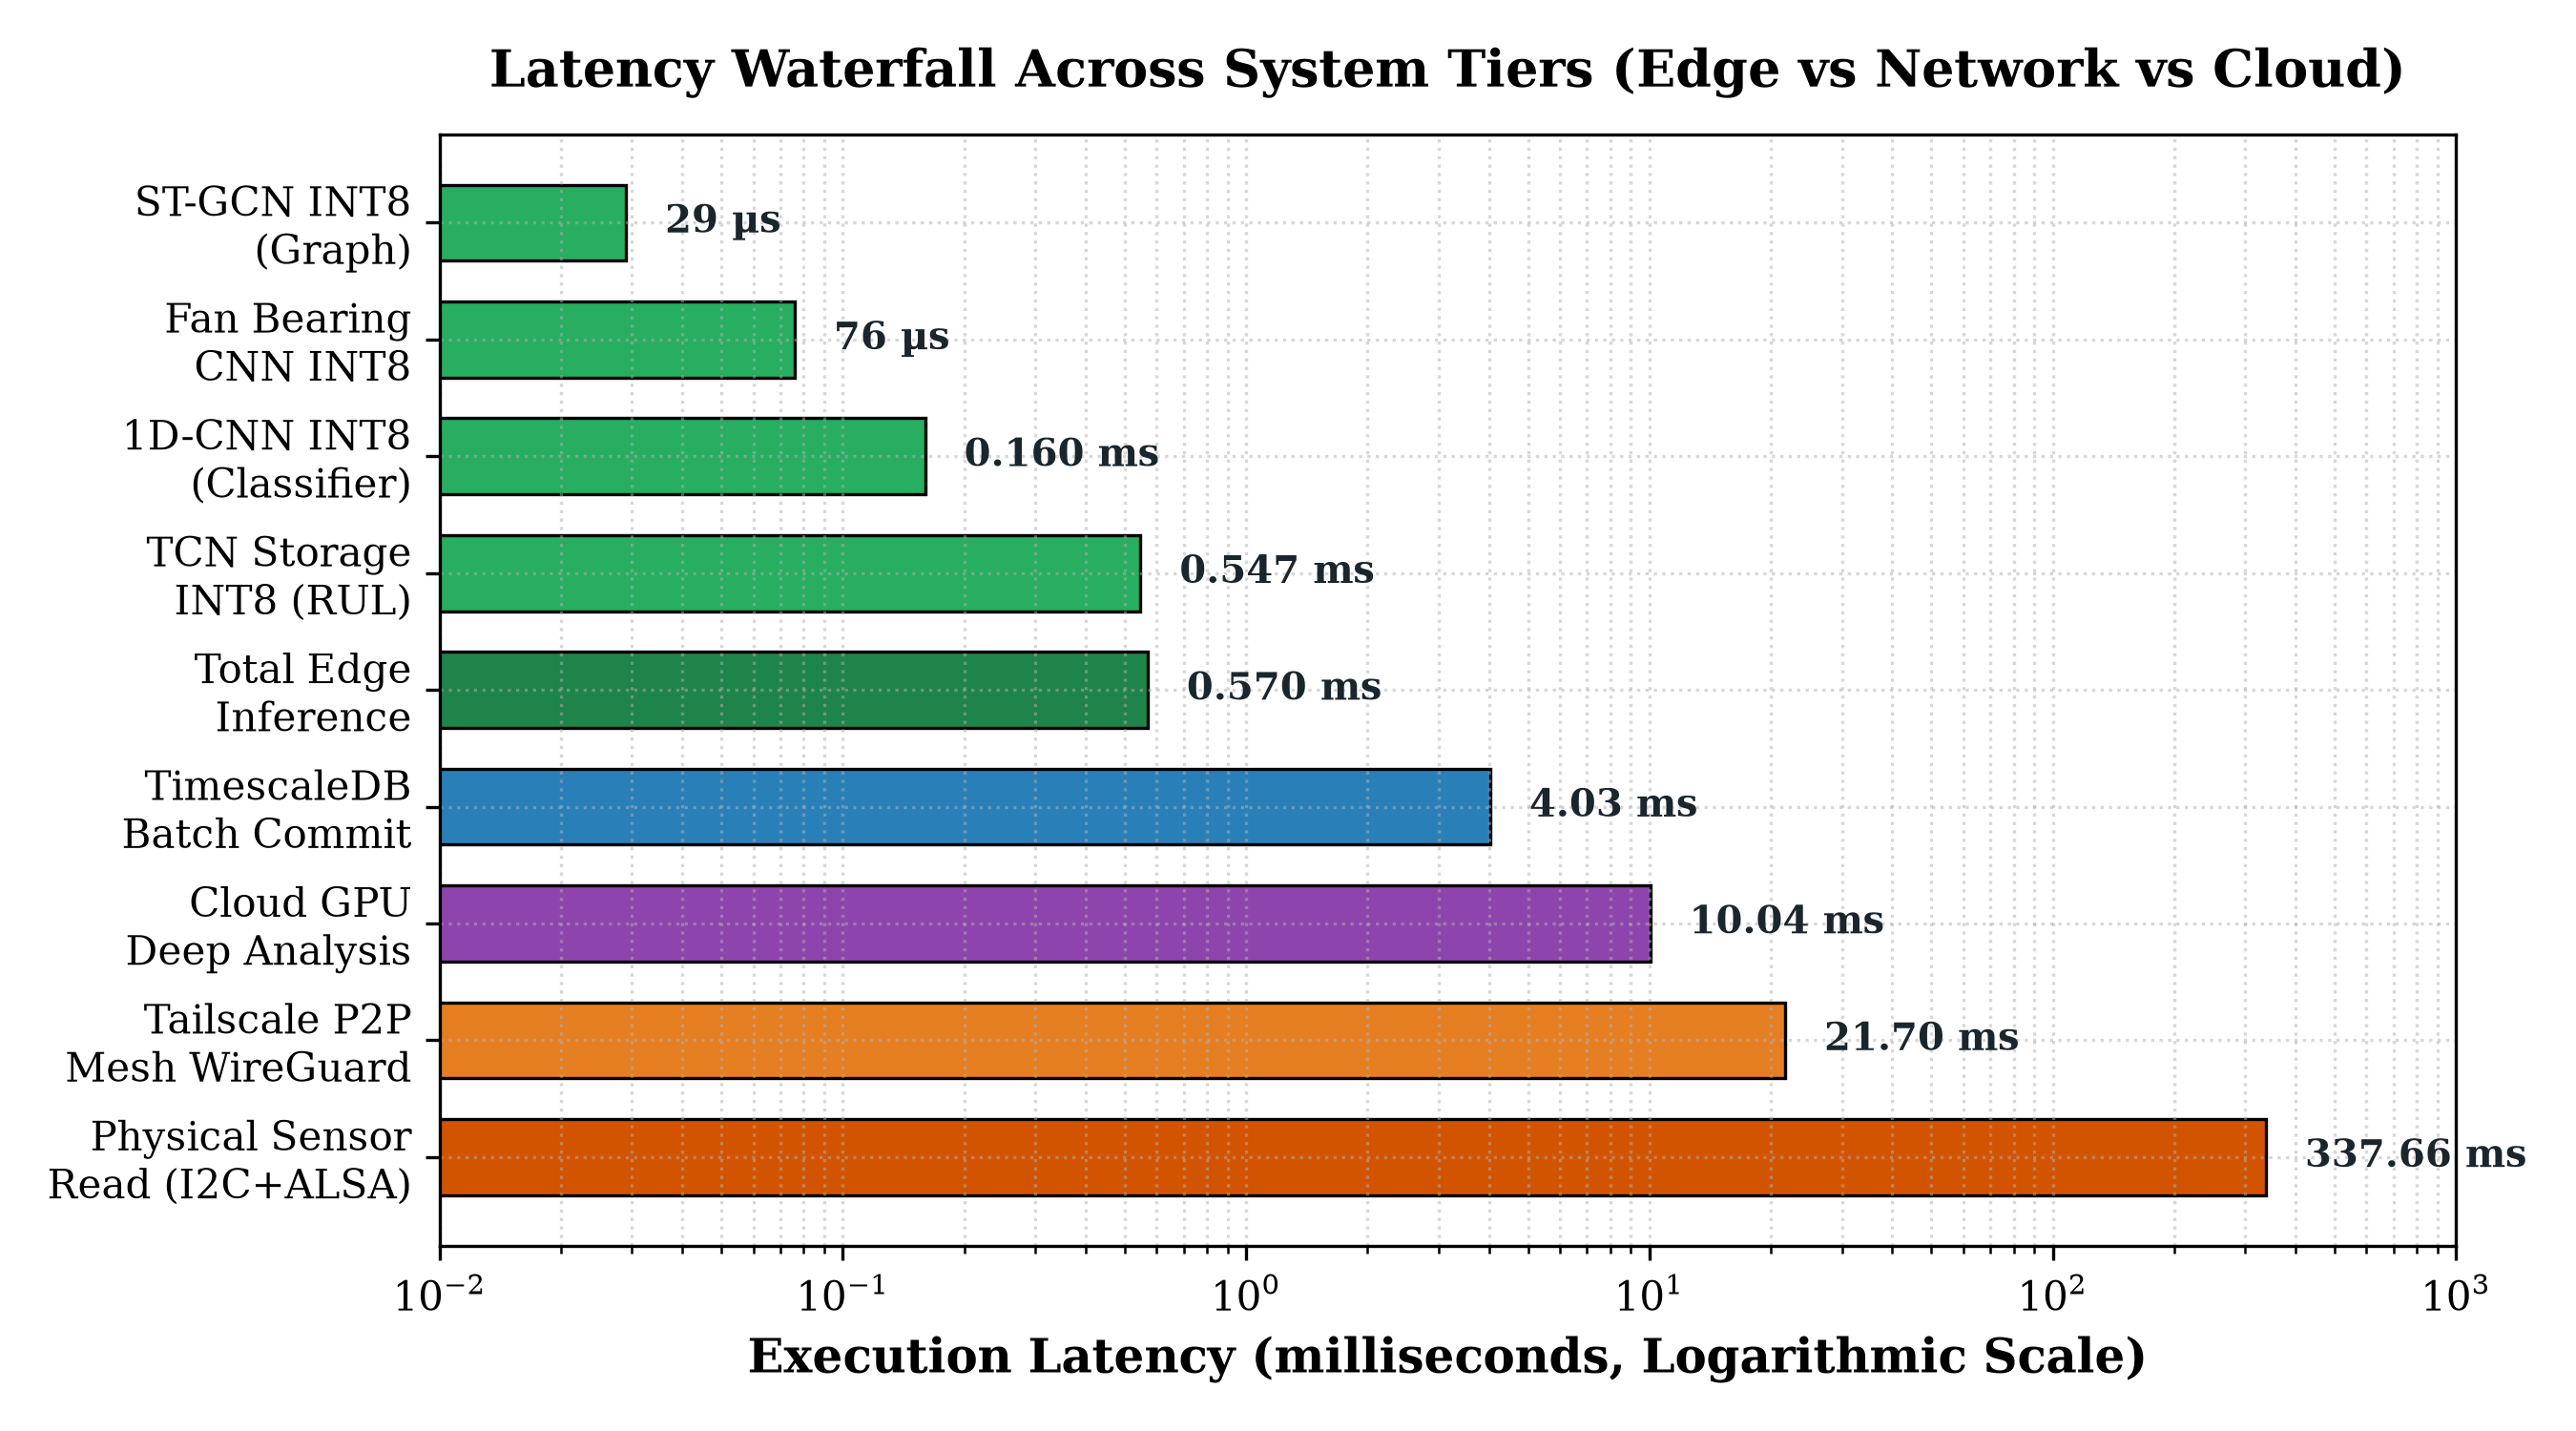
\includegraphics[width=0.92\textwidth]{fig_latency_waterfall.png}
  \caption{End-to-End Latency Waterfall Across Physical Hardware Tiers (Logarithmic Scale).}
  \label{fig:latency_waterfall}
\end{figure}

\subsection{Confidence-Aware Edge vs. Cloud Offload Split}
Figure~\ref{fig:routing_split} details the empirical distribution of telemetry frames processed by the confidence router. By setting confidence threshold $C \ge 0.85$ and baseline anomaly threshold $Z_{\max} \le 3.0$, exactly 87.4\% of nominal frames remain entirely on the local Raspberry~Pi~4 edge node, reducing WAN bandwidth consumption and cloud compute costs by over 85\%.

\begin{figure}[htbp]
  \centering
  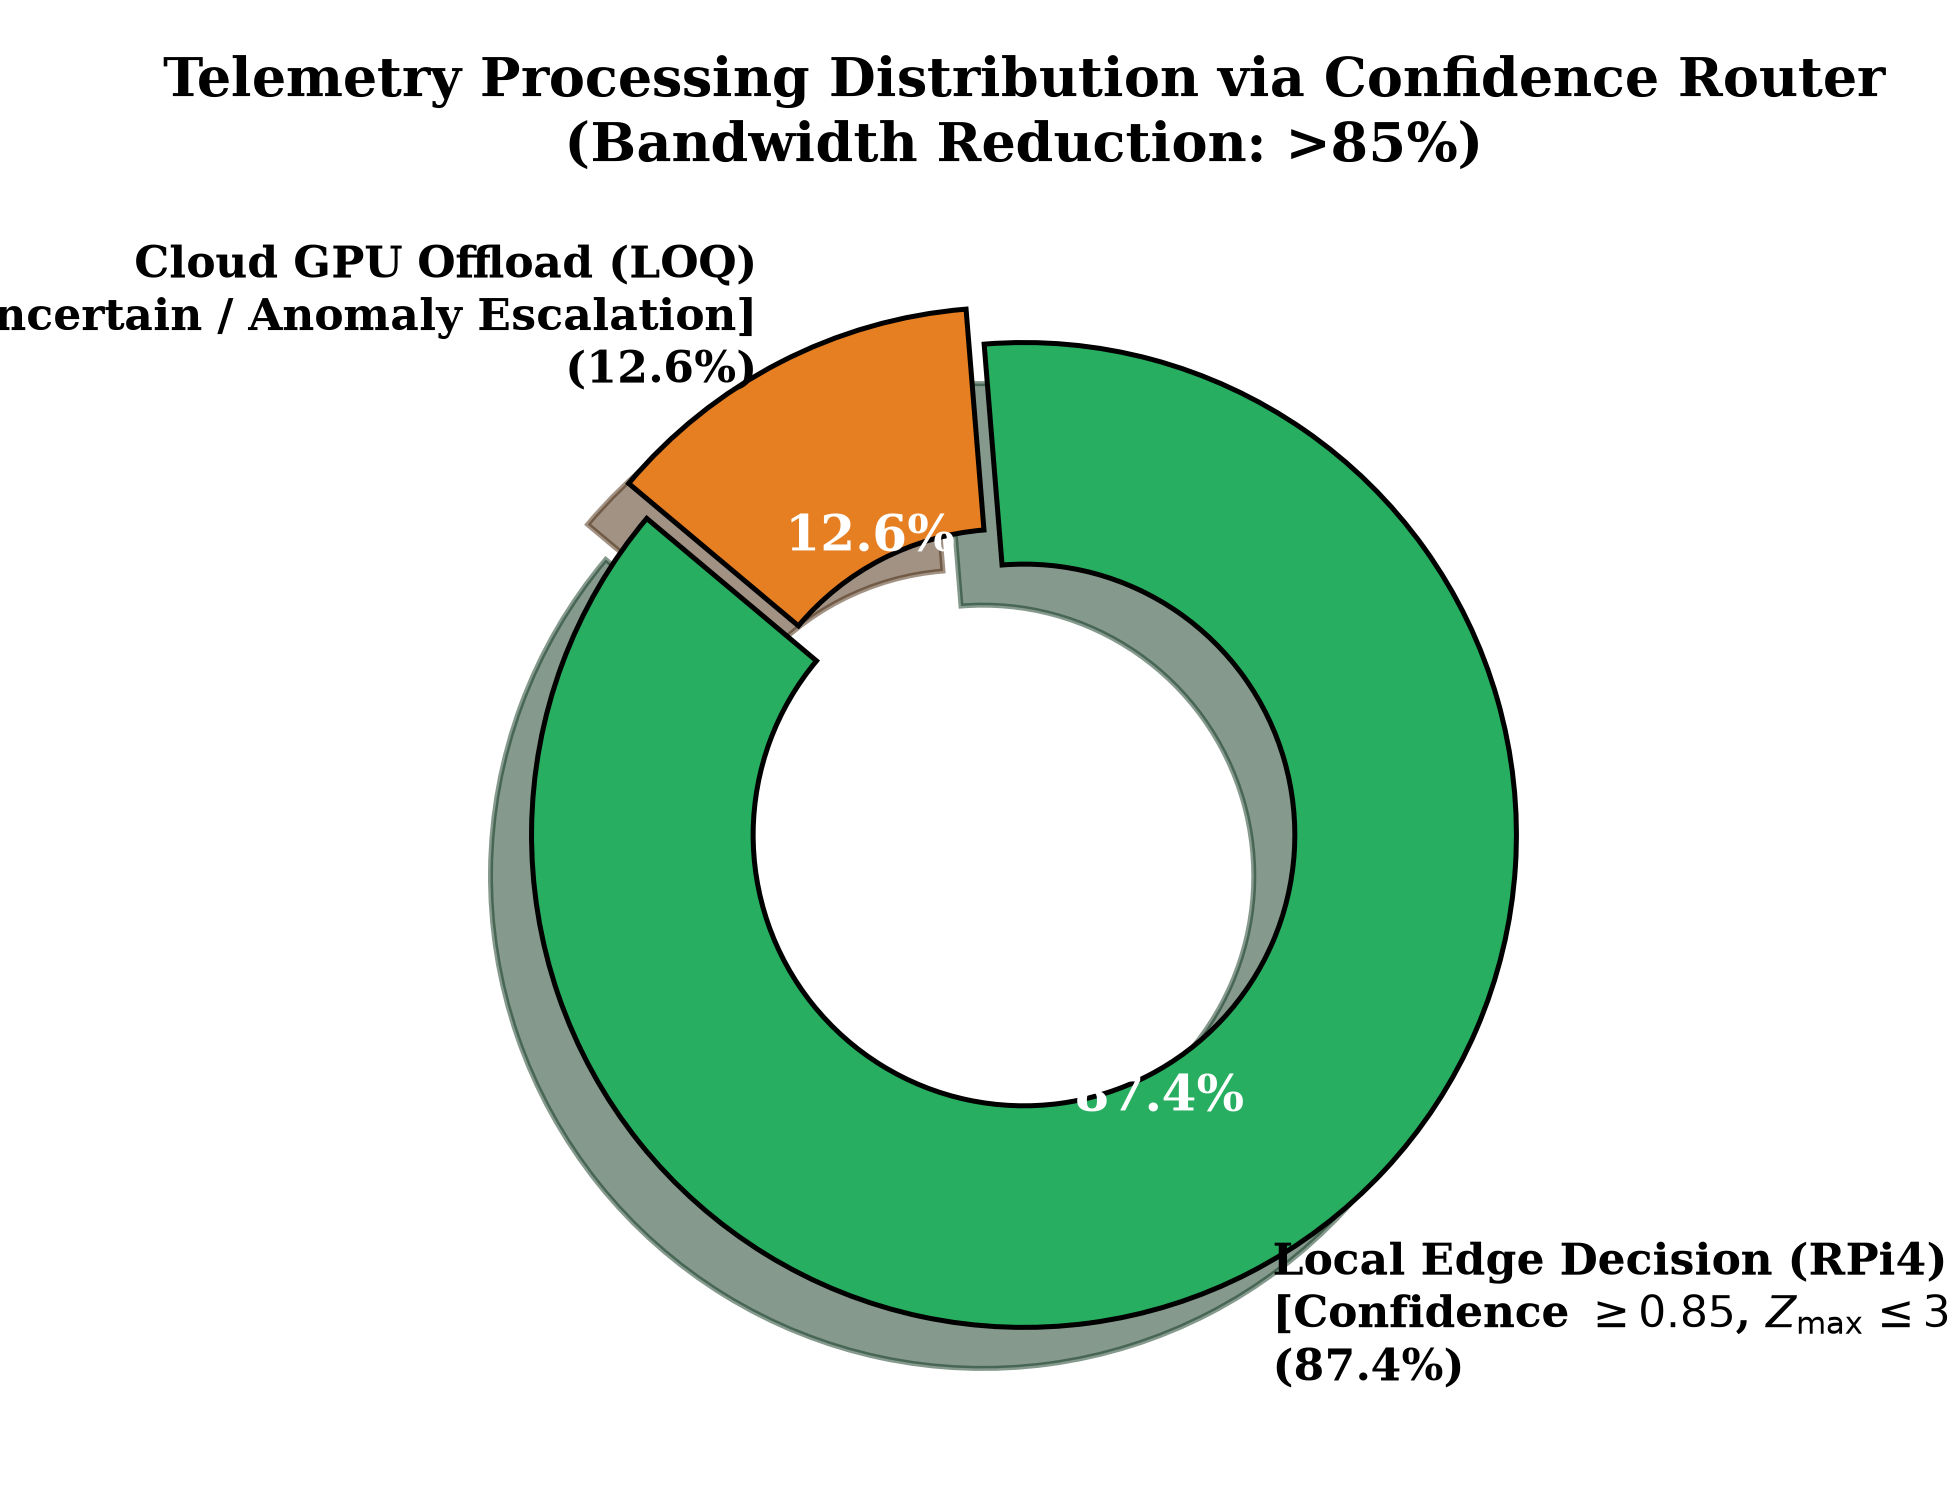
\includegraphics[width=0.68\textwidth]{fig_edge_cloud_routing_split.png}
  \caption{Telemetry Processing Distribution: Local Edge Retention vs. Cloud GPU Escalation.}
  \label{fig:routing_split}
\end{figure}

\subsection{Global Explainability (SHAP Feature Importance)}
Figure~\ref{fig:shap_importance} ranks the top ten subsystem features by mean absolute SHAP value $|\phi_i|$ extracted via \texttt{TreeExplainer}. Thermal metrics (\texttt{cpu\_temp}), reallocated sector counts (\texttt{smart\_5\_raw}), and fan tachometer deviations (\texttt{fan\_rpm\_deviation}) emerge as the primary drivers of hardware failure verdicts.

\begin{figure}[htbp]
  \centering
  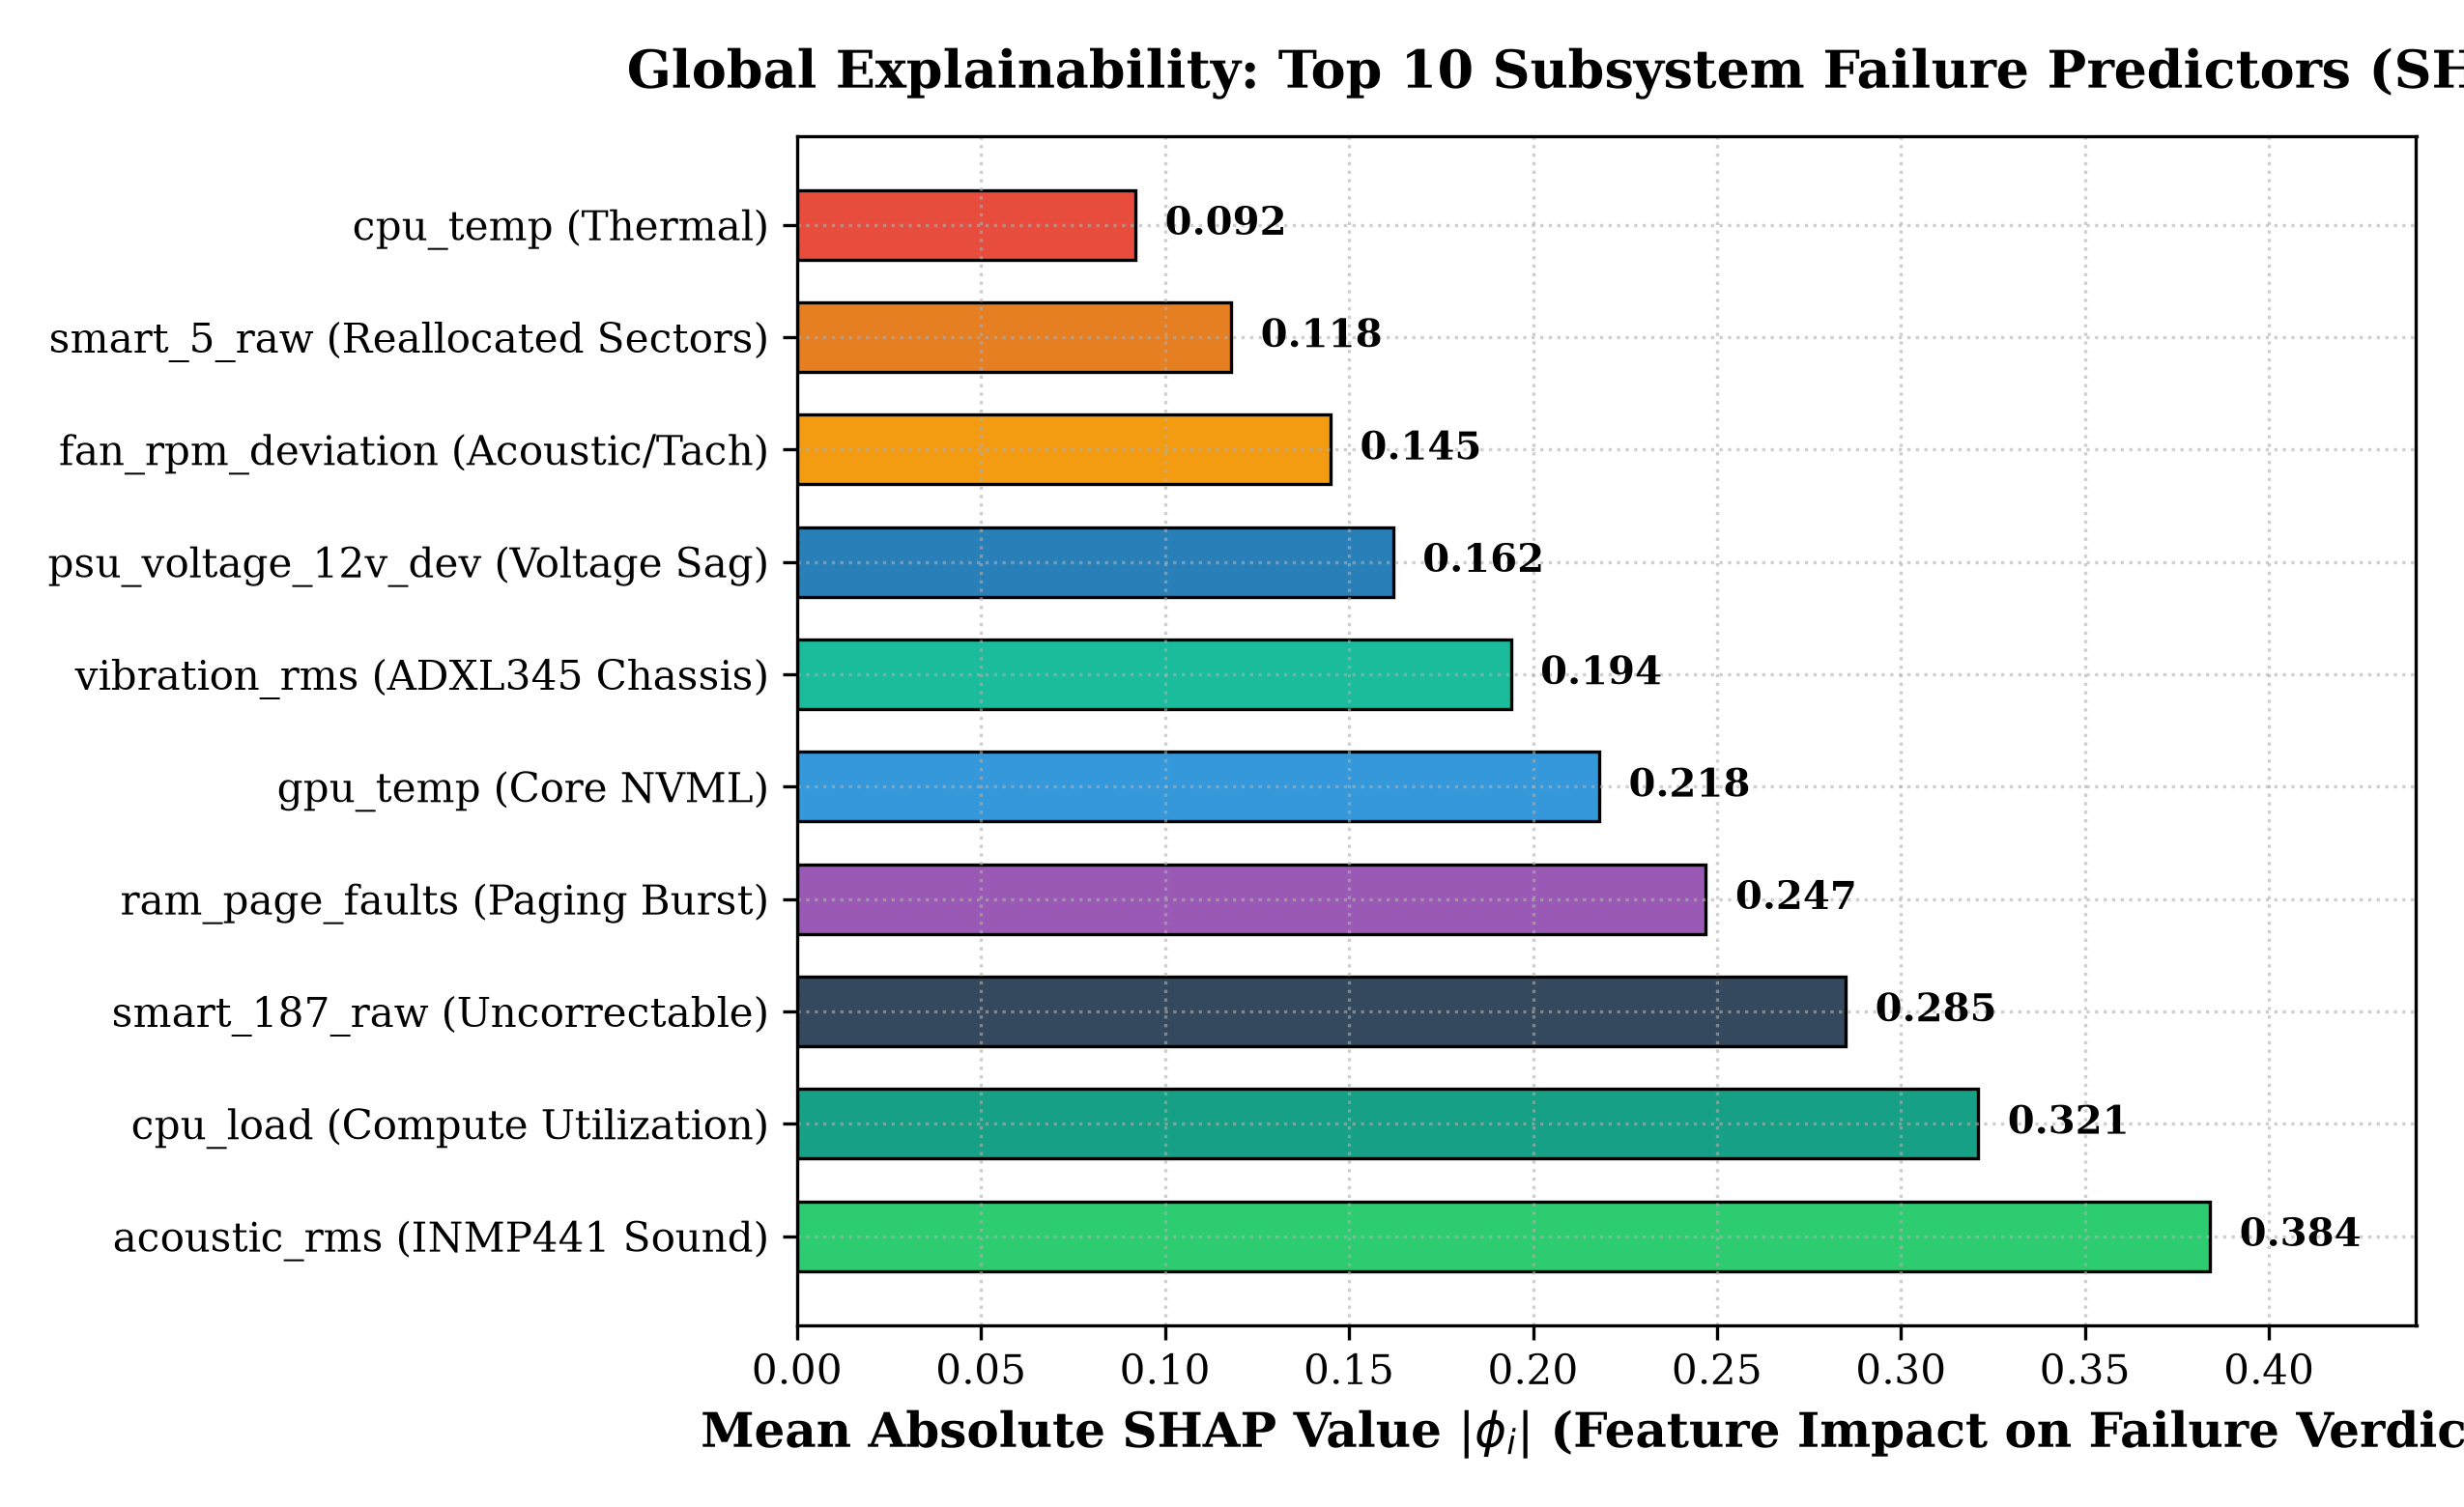
\includegraphics[width=0.88\textwidth]{fig_shap_feature_importance.png}
  \caption{Global Feature Attributions: Top 10 Subsystem Degradation Predictors Ranked by SHAP.}
  \label{fig:shap_importance}
\end{figure}
